% !TEX root = ../main.tex
% chktex-file 46
\chapter{Related Work}%
\label{sec:related}

Before combining \ac{lta} and \ac{gcr} as described in \cref{sec:intro:goals}, we first give an overview of the state-of-the-art in both fields of research.
This is done in three steps:
\begin{enumerate}
	\item We begin with an overview of the existing \ac{lta} methods for set inputs.
	\item Before the existing \ac{gcr} methods are described, we look at the graph theoretical fundamentals on which those methods are based.
	\item Using the previously introduced fundamentals, the current approaches to tackle the \ac{gcr} problem are then described.
\end{enumerate}

\section{Learning to Aggregate}%
\label{sec:related:lta}

The class of \ac{lta} problems was first described by \citet{Melnikov2016}.
There an input instance is understood as a composition $\bm{c}$ of so-called constituents $c_i \in \bm{c}$, i.e.\ as a variable-size multiset with $n = |\bm{c}|$.
The assumption in \ac{lta} problems is that for all constituents $c_i$ a local score $y_i \in \mathcal{Y}$ is either given or computable.
The set of those local scores should be indicative of the overall score $y \in \mathcal{Y}$ of the composition $\bm{c}$.
\ac{lta} problems typically require two subproblems to be solved:
\begin{enumerate}[label=\textbf{\arabic*.}]
	\item \textbf{Aggregation:}
		A variadic aggregation function $\mathcal{A}: \mathcal{Y}^{*} \to \mathcal{Y}$ that estimates composite scores has to be learned, i.e.\@ $y_i \approx \hat{y} = \mathcal{A}(y_{1}, \dots, y_{n})$.
		Typically the aggregation function $\mathcal{A}$ should be associative and commutative to fit with the multiset-structure of compositions.
	\item \textbf{Disaggregation:}
		In case the constituent scores $y_i$ are not given, they have to be derived from a constituent representation, e.g.\ a vector $x_i \in \mathcal{X}$.
		To learn this derivation function $f: \mathcal{X} \to \mathcal{Y}$, only the constituent vectors ${\{x_i\}}_{i = 1}^{n}$ and the composite score $y$ is given.
		Thus the constituent scores $y_i$ need to be \textit{disaggregated} from $y$ in order to learn $f$.
\end{enumerate}
\begin{figure}
	\centering
	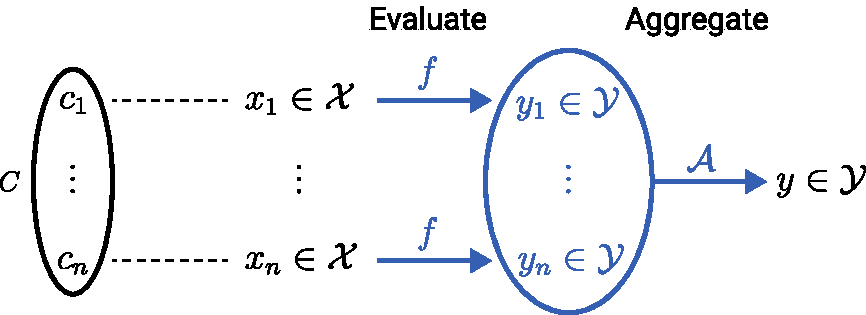
\includegraphics[width=0.7\linewidth]{gfx/related-work/lta-overview.pdf}
	\caption{Overview of the structure of LTA for multiset compositions.}\label{fig:related:lta-overview}
\end{figure}
Overall \ac{lta} can be understood as the joint problem of learning the aggregation function $\mathcal{A}$ and the local score derivation function $f$.
Two main approaches to represent the aggregation function in \ac{lta} problems have been explored.

\subsection{Uninorm-Aggregation}%
\label{sec:related:lta:uninorm}

The first approach uses \textit{uninorms}~\cite{Melnikov2016} to do so.
There the basic idea is to express composite scores as fuzzy truth assignments $y \in [0, 1]$.
Such a composite assignment $y$ is modeled as the result of a parameterized logical expression of constituent assignments $y_i \in [0, 1]$.
As the logical expression that thus effectively aggregates the constituents, a uninorm $U_{\lambda}$ is used.
Depending on the parameter $\lambda \in [0, 1]$, $U_{\lambda}$ combines a t-norm $T$ and a t-conorm $S$ which are continuous generalizations of logical conjunction and disjunction respectively.
One popular choice of norms are the so-called Łukasiewicz norms:
\begin{align}
	\text{t-norm } T(a, b) &:= \max \{ 0, a + b - 1 \}, \quad\text{t-conorm } S(a, b) := \min \{ a + b, 1 \}, \nonumber \\
	\text{uninorm } U_\lambda(a, b) &:= \begin{cases}
		\lambda T\left(\frac{a}{\lambda}, \frac{b}{\lambda}\right) & \text{if } a, b \in [0, \lambda] \\
		\lambda + (1 - \lambda) S\left(\frac{a - \lambda}{1 - \lambda}, \frac{b - \lambda}{1 - \lambda}\right) & \text{if } a, b \in [\lambda, 1] \\
		\lambda \min \{ a, b \} & \text{else}
	\end{cases}
\end{align}
At the extreme points $(0, 0)$, $(0, 1)$, $(1, 0)$ and $(1, 1)$, $T$ and $S$ coincide with the Boolean operators $\land$ and $\lor$;
the values at all other points are interpolated as shown in \cref{fig:related:logic-norms}.
The uninorm $U_\lambda$ uses the conjunctive t-norm $T$ for values below the threshold $\lambda$ and the disjunctive t-conorm $S$ for values above the threshold.
$U_\lambda$ therefore smoothly interpolates between a conjunctive and disjunctive operator with the extreme points $U_1 = T$ and $U_0 = S$.
\begin{figure}[h]
	\centering
	\begin{tikzpicture}
		\begin{axis}[
			title={t-norm $T$ ($\land$)},
			xlabel=$a$,
			ylabel=$b$,
			xlabel style={xshift=0.2cm, yshift=0.15cm},
			ylabel style={xshift=-0.2cm, yshift=0.15cm},
			tick label style={font=\scriptsize},
			width=0.33\textwidth,
			colormap = {bluered}{color(0cm) = (t_blue); color(1cm) = (t_red)}
		]
			\addplot3[
				mesh,
				samples=12,
				domain=0:1,
				domain y=0:1
			]{max(x + y - 1, 0)};
		\end{axis}
	\end{tikzpicture}
	\begin{tikzpicture}
		\begin{axis}[
			title={t-conorm $S$ ($\lor$)},
			xlabel=$a$,
			ylabel=$b$,
			xlabel style={xshift=0.2cm, yshift=0.15cm},
			ylabel style={xshift=-0.2cm, yshift=0.15cm},
			tick label style={font=\scriptsize},
			width=0.33\textwidth,
			colormap = {bluered}{color(0cm) = (t_blue); color(1cm) = (t_red)}
		]
			\addplot3[
				mesh,
				samples=12,
				domain=0:1,
				domain y=0:1
			]{min(x + y, 1)};
		\end{axis}
	\end{tikzpicture}
	\begin{tikzpicture}
		\begin{axis}[
			title={uninorm $U_{0.5}$ ($\land$/$\lor$)},
			xlabel=$a$,
			ylabel=$b$,
			xlabel style={xshift=0.2cm, yshift=0.15cm},
			ylabel style={xshift=-0.2cm, yshift=0.15cm},
			tick label style={font=\scriptsize},
			width=0.33\textwidth,
			colormap = {bluered}{color(0cm) = (t_blue); color(1cm) = (t_red)}
		]
			\addplot3[
				mesh,
				samples=12,
				domain=0:1,
				domain y=0:1
			]{(x <= 0.5 && y <= 0.5) * 0.5 * max(2 * (x + y) - 1, 0) + (x > 0.5 && y > 0.5) * (0.5 + 0.5 * min(2 * (x + y - 1), 1)) + (!(x <= 0.5 && y <= 0.5) && !(x > 0.5 && y > 0.5)) * min(x, y)};
		\end{axis}
	\end{tikzpicture}
	\caption{The Łukasiewicz norms and the corresponding uninorm for $\lambda = 0.5$.}\label{fig:related:logic-norms}
\end{figure}

Since t-norms and t-conorms are commutative and associative they can also be applied to non-empty sets of arbitrary size, i.e. $T(\{ y_1, \dots, y_n \}) = T(y_1, T(\{ y_2, \dots, y_n \}))$ with fixpoint $T(\{ y \}) = y$.
Using this extension, a uninorm $U_\lambda$ can be applied to sets which turns it into a parameterized aggregation function $\mathcal{A}_\lambda: {[0, 1]}^* \to [0, 1]$.
In this simple model the \ac{lta} aggregation problem boils down to the optimization of $\lambda$.
The \ac{lta} disaggregation problem is solved by jointly optimizing a \ac{lm}, i.e.\ the constituent scores ${\{ y_i \in [0, 1] \}}_{c_i \in \bm{c}}$ are described by $y_i = {\left( 1 + \exp(-\theta^\top x_i) \right)}^{-1}$.
Overall an \ac{lta} model is therefore described by the uninorm parameter $\lambda$ and the regression coefficients $\theta$.

\subsection{\acs*{owa}-Aggregation}%
\label{sec:related:lta:owa}

Recently \citet{Melnikov2019} have looked at an alternative class of aggregation functions.
Instead of using fuzzy logic to describe score aggregation, \ac{owa} operators were used.
\ac{owa} aggregators work by sorting the input scores and then weighting them based on their sort position, i.e.\ %
\begin{align}
	\mathcal{A}_{\lambda}(y_1, \dots, y_n) := \sum_{i = 1}^n \lambda_i y_{\pi(i)},
\end{align}
where $\lambda \in \mathbb{R}^n$ is a weight vector with ${\|\lambda\|}_1 = 1$ and $\pi$ is a sorting permutation of the input scores with $y_i < y_j \Rightarrow \pi(i) < \pi(j)$. % chktex 21
Depending on the choice of the vector $\lambda$, the \ac{owa} function $\mathcal{A}_\lambda$ can express common aggregation functions like
$\min$ (if $\lambda = (1, 0, \dots, 0)$),
$\max$ (if $\lambda = (0, \dots, 0, 1)$)
or the arithmetic mean (if $\lambda = \left(\frac{1}{n}, \dots, \frac{1}{n}\right)$).

To deal with varying composition sizes $n$, the weights ${\{ \lambda_i \}}_{i = 1}^{n}$ can however not be statically assigned.
Instead they are interpolated using a so-called \ac{bum} function $q: [0, 1] \to [0, 1]$.
It takes constituent positions that are normalized to the unit interval, i.e.\ $\frac{i}{n} \in [0, 1]$.
The \ac{bum} function $q$ is then used to interpolate a weight for any normalized sort position via $\lambda_i := q\left(\frac{i}{n}\right) - q\left(\frac{i - 1}{n}\right)$.
Because $q$ is monotone with $q(0) = 0$ and $q(1) = 1$, it always holds that ${\|\lambda\|}_1 = q(1) - q(0) = 1$. % chktex 21
Using this model, the aggregation problem boils down to optimizing the shape of $q$.

\begin{figure}[h]
	\centering
	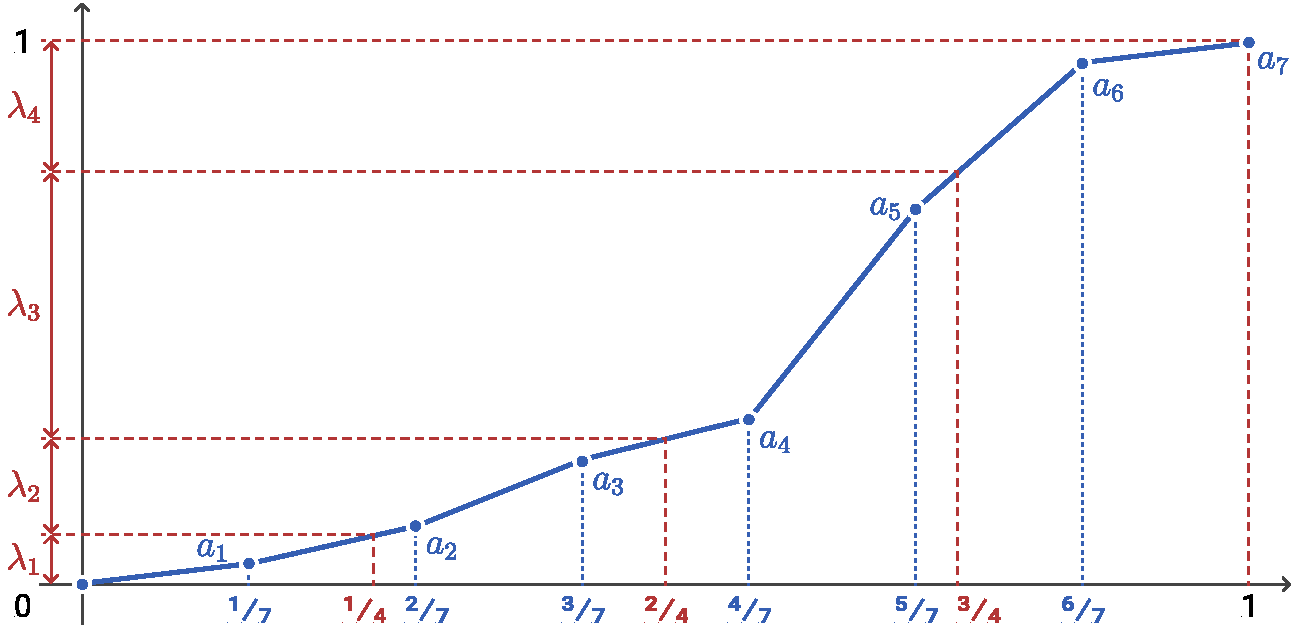
\includegraphics[width=0.75\linewidth]{gfx/related-work/bum.pdf}
	\caption[Illustration of how a \ac{bum} function is described as a linear spline and its relation to the \ac{owa} weights.]{
		Illustration of how \textcolor{t_blue}{$a$} describes \textcolor{t_blue}{$q$} and its relation to \textcolor{t_red}{$\lambda$} ($n = 4$, $m = 7$).
	}\label{fig:related:bum}
\end{figure}
In the \ac{owa} approach the \ac{bum} function $q$ is modeled as a piecewise linear spline.
This spline is described by $m+1$ points ${\left\{ \left( \frac{j}{m}, a_j \right) \right\}}_{j = 0}^{m}$, the so-called knots of the spline. % chktex 21
The curve of $q$ is obtained by linearly interpolating between neighboring knots as shown in \cref{fig:related:bum}.
If $0 = a_0 \leq a_1 \leq \cdots \leq a_m = 1$, $q$ is a \ac{bum} function.
The \ac{lta} aggregation problem is therefore solved by optimizing $a \in \mathbb{R}^{m + 1}$ under this constraint.
The disaggregation problem is tackled by adding the scores $y_1, \dots, y_M \in \mathbb{R}$ to the learnable parameters of the model where $M$ is assumed to be the finite number of constituents.
Currently the \ac{owa} approach requires all possible constituents to be part of the training dataset since it does not consider constituent features $x_i \in \mathcal{X}$ to predict the scores of previously unseen constituents.

\section{Graph Theoretical Fundamentals}%
\label{sec:related:theory}

\subsection{Graph Isomorphism Checks}%
\label{sec:related:theory:wl}

\subsection{Spectral Graph Theory}%
\label{sec:related:theory:spectral}

\section{Graph Regression and Classification}%
\label{sec:related:gcr}

The existing approaches to tackle the \ac{gcr} problem can be categorized into three main families:
\begin{enumerate*}
	\item Explicit graph embeddings,
	\item Graph kernels and
	\item Graph neural networks
\end{enumerate*}.
We will now look at the characteristics of those families and give an overview of specific methods.

\subsection{Explicit Graph Embeddings}%
\label{sec:related:gcr:embed}

The basic idea of graph embedding approaches is to map a graph $G$ to some finite vector space $\mathcal{X} = \mathbb{R}^d$.
By embedding a graph any classification or regression algorithm that works with vectors can then be applied.
There are three main types of explicit graph embedding approaches.

\subsubsection{Fingerprint embeddings}
The first works on graph embeddings were motivated by the study of chemical structures~\cite{Adamson1973}\cite{Willett1986}.
There a molecule can be interpreted as a labeled graph for which the \ac{gcr} problem corresponds to the prediction of some chemical property, e.g.\ toxicity or solubility.
Fingerprint embeddings try to find a fixed set of subgraphs $S_1, \dots, S_d$ in an input graph.
The embedding of the input graph $G$ is a binary vector $x \in {\{0, 1\}}^d$ with $x_i = \mathds{1}[\text{$S_i$ is subgraph of $G$}]$, where $\mathds{1}$ denotes the indicator function.
This simple approach requires a careful choice of subgraphs by domain experts but can still be competitive with the other more recent approaches we will look at next.
Fingerprint embeddings are for example used in multiple state-of-the-art toxicity prediction tools like RASAR~\cite{Luechtefeld2018}\cite{ToxTrack}, ProTox~\cite{Drwal2014}\cite{Banerjee2018}\cite{ProTox} or the \ac{toxTest}~\cite{TEST}.

\subsubsection{Unsupervised embeddings}
While fingerprint embeddings use a fixed set of subgraphs to characterize a given graph, unsupervised embedding methods determine relevant substructures dynamically.
One such method is \texttt{graph2vec}~\cite{Narayanan2017} which is based on the \texttt{doc2vec}~\cite{Le2014} document embedding method from \ac{nlp}.
\texttt{graph2vec} takes a set of graphs $\mathbb{G} = \{ G_1, \dots, G_N \}$ as input and finds an embedding $\varphi: \mathbb{G} \to \mathbb{R}^d$ in which graphs that share isomorphic subgraphs are mapped closer to each other than those that do not.

\subsection{Implicit Graph Embeddings via Kernels}%
\label{sec:related:gcr:kernel}

\subsection{Graph Neural Networks}%
\label{sec:related:gcr:nn}

\subsubsection{Spatial GNNs}

\subsubsection{Spectral GNNs}
